% !TeX root = ..\main.tex
\chapter{Results}

\section{Verification of derivatives}



\section{Comparison of methods}

\subsection{Advection equation}

We have chosen to start with the advection equation, as it is the simplest of the two PDEs we are considering.
Since this is a relatively easy problem, we expect all methods to be able to perform well, and it acts as a good starting point for comparison.

\subsubsection{Vanilla methods}

\begin{figure*}[h!]
    \centering
    \includesvg{loss_advection}
    \caption[Loss plot, using vanilla methods on the advection equation]{Loss plot, using vanilla methods on the advection equation.}
    \label{fig:loss_plot_kdv}
\end{figure*}

\newpage

\begin{figure*}[h!]
    \includesvg{pred_advection}
    \caption[Predictions on advection with vanilla methods]{Predictions on advection with vanilla methods}
    \label{fig:pred_kdv_vanilla}
\end{figure*}

\begin{figure*}[h!]
    \includesvg{pred_advection_imshow}
    \caption[Predictions on advection with vanilla methods]{Predictions on advection with vanilla methods}
    \label{fig:pred_kdv_vanilla_imshow}
\end{figure*}

\subsubsection{Hamiltonian Operator Network}

\subsection{Korteweg–De Vries equation}

\subsubsection{"Vanilla" methods}

\begin{figure*}[h!]
    \centering
    \includesvg{loss_kdv}
    \caption[Loss plot, using vanilla methods on KdV]{Loss plot, using vanilla methods on KdV.}
    \label{fig:loss_plot_kdv}
\end{figure*}

\begin{figure*}[h!]
    \includesvg{pred_kdv}
    \caption[Predictions on KdV with vanilla methods]{Predictions on KdV with vanilla methods}
    \label{fig:pred_kdv_vanilla}
\end{figure*}

\begin{figure*}[h!]
    \includesvg{pred_kdv_imshow}
    \caption[Predictions on KdV with vanilla methods]{Predictions on KdV with vanilla methods}
    \label{fig:pred_kdv_vanilla_imshow}
\end{figure*}

\subsubsection{Hamiltonian Neural Operator}

\begin{figure}[h!]
    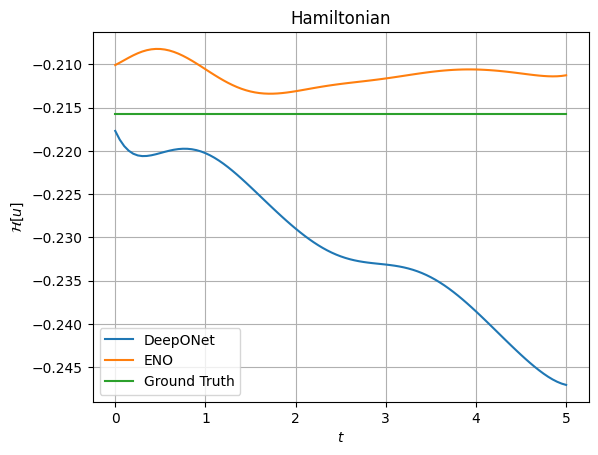
\includegraphics{ENO_Hamiltonian}
    \caption[ENO Hamiltonian]{Just a small test to see if the ENO seems to work. This looks promising to me!}
    \label{fig:ENO_Hamiltonian}
\end{figure}

\begin{table}[h]
    \centering
    \caption{Model Comparison}
    \begin{tabular}{@{}lcccc@{}}
    \toprule
    Model & \# Parameters & Time/Epoch (s) & Epochs Trained & Test Error \\
    \midrule
    DeepONet & 1,234,567 & 12.5 & 100 & 0.05 \\
    FNO & 567,890 & 8.7 & 150 & 0.03 \\
    Modified DeepONet & 1,500,000 & 15.2 & 120 & 0.02 \\ 
    HNO & 987,654 & 10.1 & 200 & 0.04 \\
    HINO & 1,234,567 & 12.5 & 100 & 0.05 \\
    \bottomrule
    \end{tabular}
    \label{tab:model_comparison}
\end{table}